\documentclass[12pt,a4paper]{article}

% Pacotes básicos e formatação
\usepackage[utf8]{inputenc}
\usepackage[portuguese]{babel}
\usepackage[T1]{fontenc}
\usepackage{geometry}
\geometry{top=3cm, bottom=2cm, left=3cm, right=2cm}
\usepackage{graphicx}
\usepackage{hyperref}
\usepackage{xcolor}
% \usepackage{svg}

% Pacotes para formatação de código
\usepackage{listings}

% Definição de cores para o código
\definecolor{codegreen}{rgb}{0,0.6,0}
\definecolor{codegray}{rgb}{0.5,0.5,0.5}
\definecolor{codepurple}{rgb}{0.58,0,0.82}
\definecolor{backcolour}{rgb}{0.95,0.95,0.92}

% Estilo padrão do código
\lstdefinestyle{mystyle}{
    backgroundcolor=\color{backcolour},   
    commentstyle=\color{codegreen},
    keywordstyle=\color{magenta},
    numberstyle=\tiny\color{codegray},
    stringstyle=\color{codepurple},
    basicstyle=\ttfamily\footnotesize,
    breakatwhitespace=false,         
    breaklines=true,                 
    captionpos=b,                    
    keepspaces=true,                 
    numbers=left,                    
    numbersep=5pt,                  
    showspaces=false,                
    showstringspaces=false,
    showtabs=false,                  
    tabsize=2
}

% Configuração específica para SQL
\lstdefinelanguage{SQL}{
  keywords={CREATE, TABLE, IF, NOT, EXISTS, INTEGER, PRIMARY, KEY, TEXT, REAL, DEFAULT, FOREIGN, REFERENCES, ON, DELETE, CASCADE, strftime},
  sensitive=true,
  comment=[l]{--},
  morestring=[b]',
}

% Configuração específica para Dart
\lstdefinelanguage{Dart}{
  keywords={class, final, int, String, double, Map, dynamic, return, factory, Future, async, await, if, for, else, void, required, this},
  sensitive=true,
  comment=[l]{//},
  morestring=[b]',
  morestring=[b]"
}

\lstset{style=mystyle}

% ==========================================
% INÍCIO DO DOCUMENTO
% ==========================================
\begin{document}

\begin{titlepage}
    \centering
    \vspace*{2cm}
    {\Huge \textbf{Relatório de Implementação}}\\[0.5cm]
    {\Large Banco de Dados e Persistência}\\[2cm]
    
    {\Large \textbf{Projeto:} PlaceZ}\\[0.5cm]
    {\large \textbf{Tecnologias:} Flutter, SQLite (\texttt{sqflite}), Shared Preferences, OpenStreetMap}\\[3cm]
    
    \vfill
    {\large \today}
\end{titlepage}

\newpage
% \tableofcontents
\newpage

\section{Estrutura do Banco de Dados (SQLite)}
O banco de dados relacional foi implementado utilizando o pacote \texttt{sqflite}. A versão atual contempla as tabelas de pessoas, locais, eventos e a relação N:N entre pessoas e locais. 

\subsection{Script de Criação (Schema)}
Correções importantes foram aplicadas no SQL para garantir compatibilidade com as versões do SQLite embarcadas no Android. Destaca-se a substituição da função \texttt{unixepoch()} por \texttt{(strftime(`\%s', `now'))} para evitar erros de sintaxe, além da adição das colunas \texttt{latitude} e \texttt{longitude} na tabela de locais.

\begin{lstlisting}[language=SQL, caption={Script de criação das tabelas.}]
-- Tabela de pessoas
CREATE TABLE IF NOT EXISTS pessoa(
  id    INTEGER PRIMARY KEY,
  nome  TEXT NOT NULL
);

-- Tabela de locais (Atualizada com coordenadas)
CREATE TABLE IF NOT EXISTS local(
  id          INTEGER PRIMARY KEY,
  nome        TEXT,
  endereco    TEXT,
  numero      INTEGER,
  complemento TEXT,
  latitude    REAL,
  longitude   REAL
);

-- Tabela de eventos
CREATE TABLE IF NOT EXISTS evento(
  id                INTEGER PRIMARY KEY,
  titulo            TEXT NOT NULL,
  descricao         TEXT,
  data_hora_inicio  INTEGER,
  data_hora_fim     INTEGER,
  criado_em         INTEGER DEFAULT (strftime('%s', 'now')),
  id_local          INTEGER,
  criado_por        INTEGER,
  FOREIGN KEY(id_local) REFERENCES local(id),
  FOREIGN KEY(criado_por) REFERENCES pessoa(id)
);

-- Tabela N:N entre pessoas e locais
CREATE TABLE IF NOT EXISTS pessoa_local(
  id_pessoa INTEGER NOT NULL,
  id_local  INTEGER NOT NULL,
  PRIMARY KEY (id_pessoa, id_local),
  FOREIGN KEY (id_pessoa) REFERENCES pessoa(id) ON DELETE CASCADE,
  FOREIGN KEY (id_local) REFERENCES local(id) ON DELETE CASCADE
);
\end{lstlisting}

\section{Camada de Modelos (Models)}
Os modelos são responsáveis por converter os objetos Dart em \texttt{Map} (para salvar no banco) e vice-versa.

\subsection{Modelo \texttt{Local}}
\begin{lstlisting}[language=Dart, caption={Modelo Local com suporte a coordenadas.}]
class Local {
  final int? id;
  final String? nome;
  final String? endereco;
  final double? latitude;
  final double? longitude;

  Local({this.id, this.nome, this.endereco, this.latitude, this.longitude});

  Map<String, dynamic> toMap() {
    return {
      'id': id,
      'nome': nome,
      'endereco': endereco,
      'latitude': latitude,
      'longitude': longitude,
    };
  }

  factory Local.fromMap(Map<String, dynamic> map) {
    return Local(
      id: map['id'] as int?,
      nome: map['nome'] as String?,
      endereco: map['endereco'] as String?,
      latitude: map['latitude'] as double?,
      longitude: map['longitude'] as double?,
    );
  }
}
\end{lstlisting}

\section{Camada de Acesso a Dados (DAOs)}
Os DAOs encapsulam as queries SQL, garantindo que a interface não acesse o banco diretamente.

\subsection{\texttt{LocalDao} (Métodos principais)}
\begin{lstlisting}[language=Dart, caption={Exemplo de métodos do LocalDao.}]
class LocalDao {
  Future<int> insert(Local local) async {
    final db = await BancoApp.instancia.database;
    return await db.insert('local', local.toMap());
  }

  Future<Local?> getById(int id) async {
    final db = await BancoApp.instancia.database;
    final maps = await db.query('local', where: 'id = ?', whereArgs: [id]);
    if (maps.isNotEmpty) return Local.fromMap(maps.first);
    return null;
  }
}
\end{lstlisting}

\section{Integrações e Funcionalidades Implementadas}
\begin{itemize}
    \item \textbf{Criação de Eventos Vinculada a Locais:} O formulário de eventos permite escolher um local já cadastrado, buscar um endereço real via API do OpenStreetMap (Nominatim) ou selecionar um ponto manualmente usando o mapa interativo (\texttt{flutter\_map}). O \texttt{id} gerado é salvo na coluna \texttt{id\_local} do evento.
    \item \textbf{Exibição no Calendário:} A tela do \texttt{TableCalendar} consome o \texttt{EventoDao.getAll()}, agrupa os eventos por dia e os destaca visualmente usando marcadores (\textit{dots}).
    \item \textbf{Busca de Locais:} A tela de pesquisa consome o \texttt{LocalDao.getAll()} e filtra dinamicamente pelo nome conforme o usuário digita.
    \item \textbf{Lista de Contatos:} CRUD completo implementado para a tabela \texttt{pessoa}.
\end{itemize}

\section{Persistência de Preferências (Shared Preferences)}
Para o tema do aplicativo, foi implementada uma camada de persistência leve (chave-valor) que não sobrecarrega o SQLite.
\begin{itemize}
    \item \texttt{TemaController}: Gerencia o estado do tema.
    \item \texttt{ThemePreferences}: Salva a cor semente (convertida para inteiro via \texttt{toARGB32()}) e o \texttt{ThemeMode} (light, dark, system).
\end{itemize}

\begin{figure}[htbp]
    \centering
    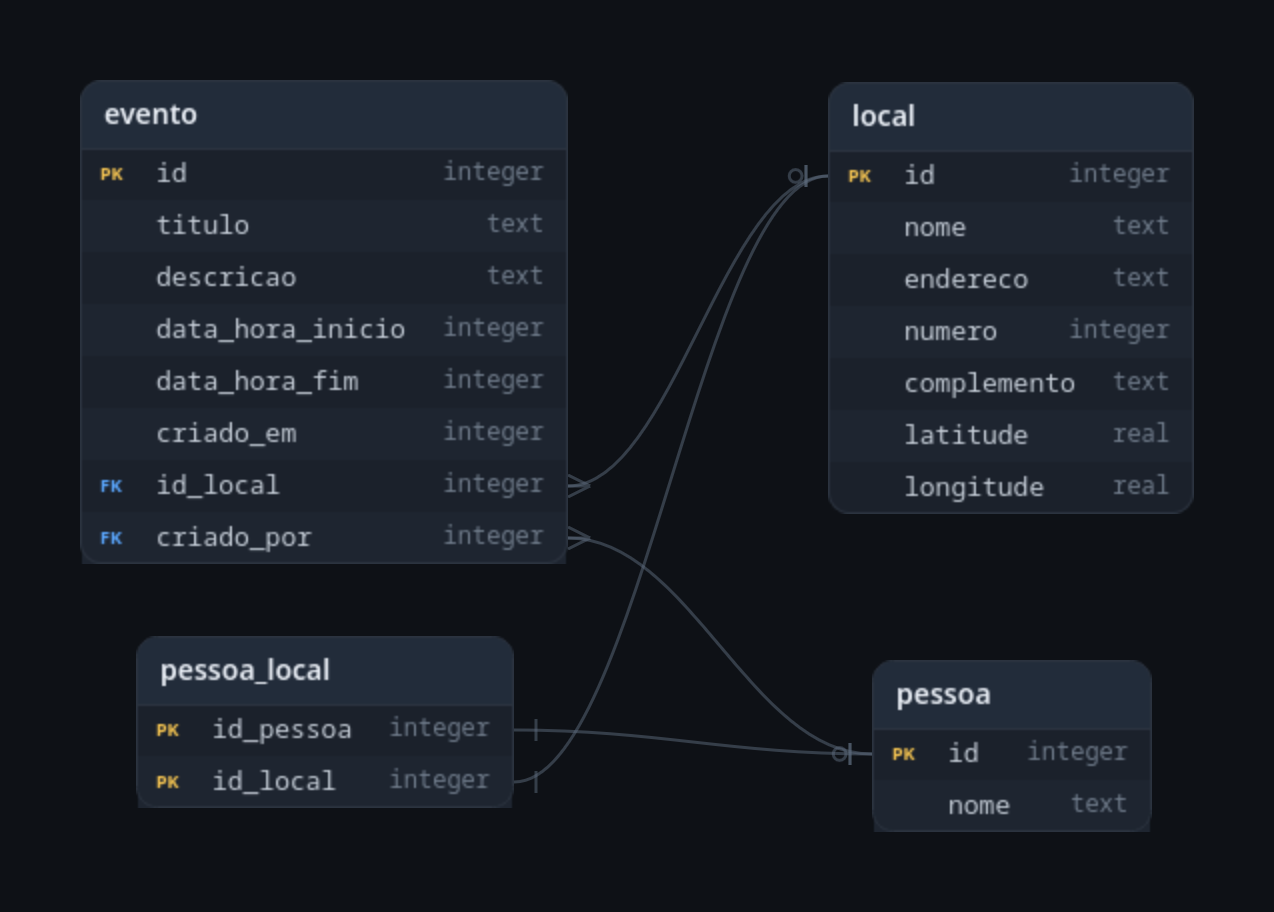
\includegraphics[width=0.9\textwidth]{schema.png}
    \caption{Diagrama de Banco de Dados}
    \label{fig:diagrama}
\end{figure}

\end{document}